\documentclass[Rapport/Rapport_main.tex]{subfiles}
\begin{document}
\section{Indledning}\label{sec:Indledning}
\subsection{Motivation og kontekst}
Beer Pong er et spil, der ofte udgør samlingspunktet ved festlige lejligheder og i sociale sammenhænge. Alkoholindtag og konkurrencer hænger uløseligt sammen, og Beer Pong formår at kombinere disse på en måde, som har gjort det til et af tidens mest populære og udbredte drukspil.\cite{drinking_research}\\\\
Beer Pong findes i forskellige varianter, men fællesnævneren for mange af spillene er simple og primitive borde. Det medfører ofte, at der opstår tvivl omkring spillets score, og om en given kop er ramt eller ej. Da det er brugernes eget ansvar at styre spillets gang, hersker der ofte udbredt forvirring. Der er således behov for et produkt, som giver visuel respons og hjælper med at vise spillets status.
\\\\Dette projektarbejde tager udgangspunkt i projektoplægget til 3. semester E/IKT\cite{Universitet2018}. Der arbejdes derfor efter en Scrum baseret proces, hvor semesterets kurser integreres. Formålet er at implementere og teste et udviklingsprojekt, som kombinerer både HW og SW.

\subsection{Hvad er og kan vores system?}
Systemet som ønskes udviklet er en forbedret og interaktiv udgave af et Beer Pong bord. For at sikre en forbedret brugeroplevelse er der lagt stor vægt på, at bordet skal give spillerne en form for visuel feedback. Dette skal blandt andet komme fra belysning under kopperne. Det skal desuden detekteres om en kop er placeret, og om den er ramt af en bordtennisbold.\\\\Via et møntindkast skal bordet modtage danske 5-kroner. Når den korrekte mønt detekteres, skal bordet forsyne spillerne med en bordtennisbold.\\\\For at sikre en endnu større grad af brugerinteraktion, skal spillerne indtaste brugernavne, holdnavne og holdfarve på en hjemmeside. Holdfarven kommer til udtryk i lysene under kopperne, mens navnene kommer til at fremgå af et display. Dette display skal desuden vise antallet af tilbageværende kopper, og det opdateres løbende under spillet. Foruden underholdningsværdien sikrer det, at alle kan følge med i spillets status, og at overblikket bevares. Det vil være oplagt at anbringe bordet et offentligt sted som en bar eller en klub, hvor man ønsker den komplette Beer Pong oplevelse.

\subsection{Projektformulering}
Målet for dette projekt er at udarbejde en funktionel prototype af et Beer Pong bord. Bordet skal være baseret på en indlejret Linux platform og PSoC platform. Det skal detektere indsatte mønter, anbringelse og fjernelse af kopper samt hændelsen, at en bordtennisbold rammer ned i en kop. Desuden skal det kunne dispensere bordtennisbolde. Bordet skal have mindst seks kopholdere med lys under hver kop. Det skal være muligt at tilgå en hjemmeside og indtaste holdnavne, brugernavne og holdfarver. Holdfarver skal fremgå af farven på lyset under kopperne, og navnene skal vises på et display. Display viser desuden holdenes score og opdateres løbende under spillet. Det samlede system skal således kombinere sensorer, aktuatorer og brugerinterfaces i et interaktivt og underholdende Beer Pong bord for at sikre den bedst mulige brugeroplevelse.

\subsubsection{Skitse af system}
Figur \ref{fig:system_skitse} viser en grafisk repræsentation af systemet. På figuren er vist et fuldt bord med to Playersides og et Display i midten. Hver Playerside består af seks Cupholders, som hver indeholder Cup lights og Cup sensor. Ball dispenser indeholder dispenser og møntindkast.

\begin{figure}[H]
    \centering
    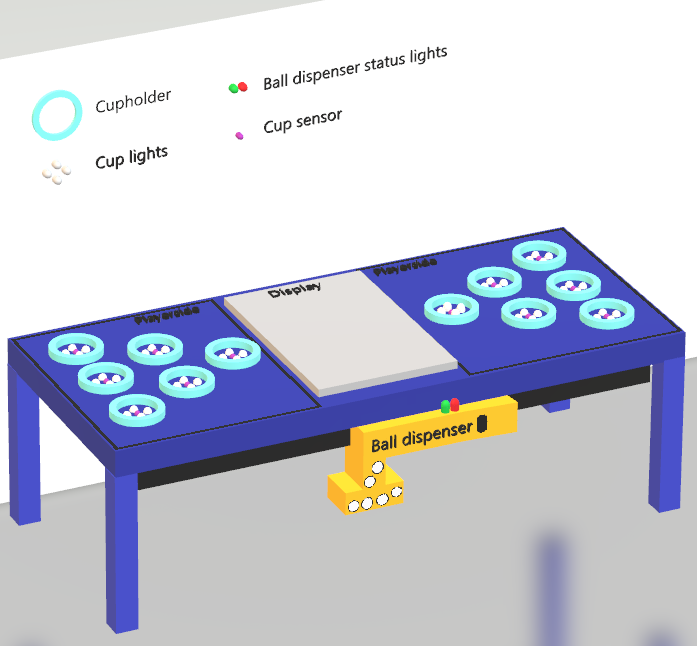
\includegraphics[width=0.9\textwidth]{Rapport/Indledning/graphics/system_skitse.png}
    \caption{Skitse af Beer Pong Table}
    \label{fig:system_skitse}
\end{figure}

\end{document}